\documentclass[conference]{IEEEtran}

% ----------------------------
% Packages
% ----------------------------
\usepackage[utf8]{inputenc}
\usepackage{amsmath, amssymb, amsthm}
\usepackage{graphicx}
\usepackage[bookmarks=true,hidelinks]{hyperref}
\usepackage{cite}
\usepackage{booktabs}
\usepackage{multirow}
\usepackage{tikz}
\usepackage{etoolbox}
\usepackage{enumerate}
\usepackage[most]{tcolorbox}
\tcbuselibrary{theorems}

\newtheorem{definition}{Definition}[section]

\tcolorboxenvironment{definition}{
  colback=blue!5!white,
  colframe=blue!30!black,
  boxrule=0.8pt,
  arc=2mm,
  left=1mm,
  right=1mm,
  top=1mm,
  bottom=1mm,
  enhanced,
  sharp corners,
  fonttitle=\bfseries,
  title style={font=\bfseries},
  before skip=0.6em, after skip=0.6em,
}

\newtheorem{proposition}{Proposition}[section]

\tcolorboxenvironment{proposition}{
  colback=green!5!white,
  colframe=green!30!black,
  boxrule=0.8pt,
  arc=2mm,
  left=1mm,
  right=1mm,
  top=1mm,
  bottom=1mm,
  enhanced,
  sharp corners,
  fonttitle=\bfseries,
  title style={font=\bfseries},
  before skip=0.6em, after skip=0.6em,
}

\tcolorboxenvironment{proof}{
    colback=red!5!white,
    colframe=red!30!black,
    boxrule=0.8pt,
    arc=2mm,
    left=1mm,
    right=1mm,
    top=1mm,
    bottom=1mm,
    enhanced,
    sharp corners,
    fonttitle=\bfseries,
    title style={font=\bfseries},
    before skip=0em, after skip=0.6em,
}

\newtheorem{theorem}{Theorem}[section]
\newtheorem{lemma}{Lemma}[section]

\tcolorboxenvironment{lemma}{
    colback=cyan!5!white,
    colframe=cyan!30!black,
    boxrule=0.8pt,
    arc=2mm,
    left=1mm,
    right=1mm,
    top=1mm,
    bottom=1mm,
    enhanced,
    sharp corners,
    fonttitle=\bfseries,
    title style={font=\bfseries},
    before skip=0.6em, after skip=0.6em,
}

\newtheorem{corollary}{Corollary}[section]

\newenvironment{note}{\par\color{teal}\begin{quote}\textbf{Note:}}{\end{quote}}

\tcbset{theorem style=plain}
\tcbset{coltitle=black, fonttitle=\bfseries}

% ----------------------------
% Title
% ----------------------------
\title{\huge Graph-Based Analysis of Solution Spaces in the Game \textit{Diplomatico}}

\author{
    \IEEEauthorblockN{Filippo Garagnani}
    \IEEEauthorblockA{
        Dipartimento di Ingegneria "Enzo Ferrari" \\
        Università degli Studi di Modena e Reggio Emilia \\
        \texttt{298707@studenti.unimore.it}
    }
}

\begin{document}
\maketitle

\begin{abstract}
The game of \textit{Diplomatico} (also known as 'The 100 Squares Puzzle' or 'Hopido' \cite{hopido}) has been studied during the last decades. 
The few results found are limited to determining whether the game is solvable or not for certain given constraints.
However, to the best of our knowledge, no one has ever tried to analyze different approaches to explore the solution space in its entirety.
In this work, we model the game as a graph where nodes represent squares and edges represent valid moves between these cells. 
We apply various graph analytics techniques to uncover structural properties of the solution space, identify key states, and explore potential strategies for solving the game.
\end{abstract}

% ----------------------------
% Sections
% ----------------------------

\section{Introduction}
The game of \textit{Diplomatico} is a combinatorial puzzle game, usually played on a square grid.
The goal of the game is to fill the grid with numbers, by placing them according to the following rules:
\begin{enumerate}
    \item The number $1$ can be placed on any available square.
    \item The number $i > 1$ must be placed either at a distance of $3$ horizontally or vertically, or at a distance of $2$ diagonally from the square containing the number $i-1$.
    \item If the number $i$ cannot be placed, the game ends.
\end{enumerate}

An example of valid moves is shown in Figure \ref{fig:example_moves}.
\begin{figure}[ht]
\centering
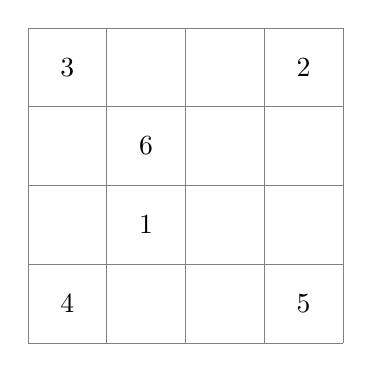
\begin{tikzpicture}
  \draw[step=1cm,gray,very thin] (0,0) grid (4,4);
  \node at (1.5,1.5) {$1$};
  \node at (3.5,3.5) {$2$};
  \node at (0.5,3.5) {$3$};
  \node at (0.5,0.5) {$4$};
  \node at (3.5,0.5) {$5$};
  \node at (1.5,2.5) {$6$};
\end{tikzpicture}
\caption{A $4 \times 4$ grid following the rules of \textit{Diplomatico}. The number $2$ is placed diagonally from $1$; while the number $3$ is placed horizontally from $2$.}
\label{fig:example_moves}
\end{figure}

As it can be seen, the requirement of a square grid is completely arbitrary. The game could be also played on rectangular grids with or without 'blocked' cells (i.e., squares which are not available).

Some very simple results are known about the game. 
For example, it has been shown that the game is unsolvable for square grids of size $4 \times 4$ or smaller - except for the trivial case in which the grid is of size $1 \times 1$ (see Figure \ref{fig:trivial_case}).

\begin{figure}[ht]
\centering
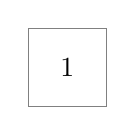
\begin{tikzpicture}
  \draw[step=1cm,gray,very thin] (0,0) grid (1,1);
  \node at (0.5,0.5) {$1$};
\end{tikzpicture}
\caption{The trivial case of a $1 \times 1$ grid.}
\label{fig:trivial_case}
\end{figure}

The game can be easily modeled as a graph. Each square of the grid is represented as a node; each available 'move' (i.e., a transition from a square to another according to the game rules) is represented as a directed edge between two nodes.
This representation allows us to apply various graph analytics techniques to analyze not only the solution space, but also the most effective way to determine a solution to the game.

\section{Preliminaries}
The following definitions are used throughout this work. The main case being considered is the one in which the game grid is rectangular and doesn't have any cell blocked.

\begin{definition}{Board Graph}{}
\label{def:board_graph}

Given a board of size $n \times m$ (with $n, m \in \mathbb{N}$), the \textbf{Board Graph} of size $n \times m$ is an undirected graph $\mathfrak{G}_{n \times m} = (V, E)$, where:
$$
    V = \{v_{i,j},\;i = 1,\,\dots,\,n \land \, j = 1,\,\dots,\,m\}
$$
and where the following condition holds:
\begin{align*}
\forall e = \{v_{i,j},\;v_{k,\ell}\} \in E,\quad&(|i - k| = 3 \land j = \ell) \\
\lor\,& (|j - \ell| = 3 \land i = k) \\
\lor\,& (|i - k| = |j - \ell| = 2)
\end{align*}

\end{definition}

Of course, the node $v_{ij}$ will represent the square located at row $i$ and column $j$ of the original grid of the game. 
The condition required for the edge set $E$ ensures that only legal moves are present as undirected arcs in a Board Graph. The edges are undirected because, of course, the movement rules are perfectly simmetrical (i.e., being able to move from cell $A$ to cell $B$ means that it's also possible to move from cell $B$ to cell $A$).

\begin{definition}{Winning Path}{} \label{def:winning_path}
Given a Board Graph $\mathfrak{G}_{n \times m} = (V, E)$, a \textbf{Winning Path} is an Hamiltonian Path in $\mathfrak{G}_{n \times m}$.
Specifically, an Hamiltonian Path is a sequence of vertices $\mathfrak{h} = (v^1,\,v^2,\,\dots,\,v^{n \times m})$ such that:
$$
    \forall \ell = 1,\,\dots,\,k-1,\;\; \{v^\ell, v^{\ell+1}\} \in E
$$
and such that:
$$
    \forall v \in V,\;\; \exists!\, v^\ell \in \mathfrak{h} : v^\ell = v
$$
\end{definition}

An Hamiltonian Path is simply, as the Definition \ref{def:winning_path} gives, a path in the graph that visits every node exactly once.

\begin{definition}{Solvability}{}
\label{def:solvability}

Given a Board Graph $\mathfrak{G}_{n \times m}$, it is said to be \textbf{solvable} if:
\begin{align*}
    \exists &\mathfrak{h} = (v^1,\,v^2,\,\dots,\,v^{n \times m}) : \\
            &\mathfrak{h} \text{ is a Winning Path in } \mathfrak{G}_{n \times m}.
\end{align*}
\end{definition}

Definition \ref{def:solvability} simply states that a Board Graph is solvable if it contains at least one Hamiltonian Path; that is, if there is a way to start from a node (i.e., a cell in the game of \textit{Diplomatico}), and to be able to reach every other node - exactly once - by following the game rules. 

Simply from the Definitions \ref{def:board_graph}-\ref{def:solvability}, it is possible to prove the following Proposition.

\begin{proposition}{Unsolvability of $\mathfrak{G}_{4 \times 4}$}{}
\label{prop:unsolvability_4x4}

The Board Graph $\mathfrak{G}_{4 \times 4}$ is unsolvable.
\end{proposition}
\begin{proof}
We can prove the unsolvability of $\mathfrak{G}_{4 \times 4}$ by contradiction. Assume that there exists a Winning Path $\mathfrak{h} = (v^1,\,v^2,\,\dots,\,v^{16})$ in $\mathfrak{G}_{4 \times 4}$. 

Since $\mathfrak{h}$ is a Hamiltonian Path, it must visit every node exactly once.
Consider the nodes in the center of the board - specifically, vertices $v_{2,2},\,v_{2,3},\,v_{3,2},\,v_{3,3}$ (see Figure \ref{fig:dim_unsolvability_4x4}).
Being $\mathfrak{G}_{4 \times 4}$ a Board Graph, the conditions for edges linking those vertices can be explicitly determined (focusing, for the time being, on $v_{2,2}$):
\begin{align*}
    &\forall e = \{v_{2,2},\;v_{i,j}\} \in E,\\
    &(|2 - i| = 3 \land 2 = j) \implies v_{i,j} \in \{v_{5,2},\,v_{-1,2}\}\\
    &(|2 - j| = 3 \land 2 = i) \implies v_{i,j} \in \{v_{2,5},\,v_{2,-1}\}\\
    &(|2 - i| = |2 - j| = 2) \implies v_{i,j} \in \{v_{0,0},\,v_{0,4},\,v_{4,0},\,v_{4,4}\}
\end{align*}
However, of the 'suggested' nodes above, only $v_{4,4}$ is actually present in $\mathfrak{G}_{4 \times 4}$ (the others are to consider 'out of bounds').
This means that the node $v_{2,2}$ can only be connected to $v_{4,4}$, implying that it must be either the first or the last node in the Winning Path $\mathfrak{h}$ (since it has degree $1$).
The same reasoning can be applied to the other three 'central' nodes; this means that four nodes must either be first or last in the path. This is not possible, hence the contradiction.

\end{proof}

\begin{figure}[ht]
\centering
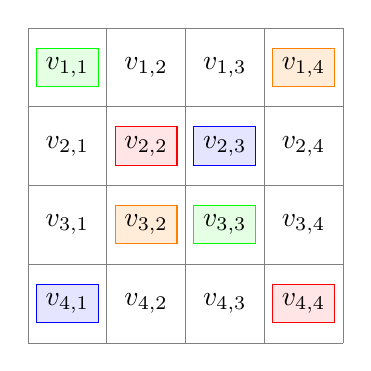
\begin{tikzpicture}
  \draw[step=1cm,gray,very thin] (0,0) grid (4,4);
  \foreach \x in {1,2,3,4} {
    \foreach \y in {1,2,3,4} {
        \ifnum\x=\y
            \pgfmathparse{mod(\x,2)==0}
            \ifnum\pgfmathresult=1
                \node[fill=red!10, draw=red] at (\x-0.5,4.5-\y) {$v_{\y,\x}$};
            \else
                \node[fill=green!10, draw=green] at (\x-0.5,4.5-\y) {$v_{\y,\x}$};
            \fi
        \else
            \pgfmathparse{\x+\y==5}
            \ifnum\pgfmathresult=1
                \pgfmathparse{mod(\x,2)==0}
                \ifnum\pgfmathresult=1
                    \node[fill=orange!15, draw=orange] at (\x-0.5,4.5-\y) {$v_{\y,\x}$};
                \else
                    \node[fill=blue!10, draw=blue] at (\x-0.5,4.5-\y) {$v_{\y,\x}$};
                \fi
            \else
                \node at (\x-0.5,4.5-\y) {$v_{\y,\x}$};
            \fi
        \fi
    }
  }
\end{tikzpicture}
\caption{The board representing the graph $\mathfrak{G}_{4 \times 4}$. In corresponding colors, the only possible edges from each central node.}
\label{fig:dim_unsolvability_4x4}
\end{figure}

The following Definition and Proposition will give a sense to the complexity of the game, and to the main focus of the work.

\begin{definition}{Numbers of Solutions}{}
\label{def:number_of_solutions}

Given a Board Graph $\mathfrak{G}_{n \times m}$, the \textbf{Number of Solutions} $\mathbf{N}(\mathfrak{G}_{n \times m})$ is defined as:
$$
    \mathbf{N}(\mathfrak{G}_{n \times m}) = |\{\mathfrak{h} : \mathfrak{h} \text{ is a Winning Path in } \mathfrak{G}_{n \times m}\}|
$$

\end{definition}

\begin{proposition}{Bounds on $\mathbf{N}(\mathfrak{G}_{n \times m})$}{}
\label{prop:bounds_number_of_solutions}

Given a Board Graph $\mathfrak{G}_{n \times m}$, with $n, m \ge 5$:
$$
    4^{\lfloor{\frac{n}{5}}\rfloor \lfloor{\frac{m}{5}}\rfloor} \le \mathbf{N}(\mathfrak{G}_{n \times m}) < 7^{nm - 1}
$$
\end{proposition}
\begin{proof}
    \textbf{Upper Bound.} 
        Any winning path $\mathfrak{h}$ must pass from a 'corner' node (i.e., $v_{1,1},\,v_{1,m},\,v_{n,1},\,v_{n,m}$). By evaluating the possibilities, it can be easily determined that only three edges are connected to any corner node.
        \begin{align*}
            &\forall e = \{v_{1,1},\;v_{i,j}\} \in E, \\
            &(|1 - i| = 3 \land 1 = j) \implies v_{i,j} \in \{v_{4,1},\,v_{-2,1}\} \\
            &(|1 - j| = 3 \land 1 = i) \implies v_{i,j} \in \{v_{1,4},\,v_{1,-2}\} \\
            &(|1 - i| = |1 - j| = 2) \implies \\
            &\quad\quad v_{i,j} \in \{v_{3,3},\,v_{3,-1},\,v_{-1,3},\,v_{-1,-1}\}
        \end{align*}
        In this specific case, the only possible adjacent nodes are $v_{4,1},\,v_{1,4},\,v_{3,3}$. The same reasoning applies to the other corner nodes.

        Moreover, the start node - in the general scenario - will have at most $8$ edges connected to it (assuming, from the previous verification, that each node is valid). Every other node, however, will have at most $7$: surely, the edge chosen to reach it should not be considered, otherwise the Winning Path wouldn't be Hamiltonian.
        This means that, combinatorially speaking:
        $$
            \mathbf{N}(\mathfrak{G}_{n \times m}) \leq 8 \cdot 3^4 \cdot 7^{nm - 5} < 7^{nm - 1}
        $$
\end{proof}
The more complex proof of the lower bound is given in Appendix \ref{appendix:proof_lower_bound}.

The derived bounds demonstrate that the number of solutions increases exponentially with the board's size. This exponential growth renders exhaustive search methods infeasible for larger boards, emphasizing the necessity for more efficient algorithms and heuristics to navigate the solution space effectively. 
Furthermore, identifying even a single solution is a challenging task. The subsequent sections will delve into different search strategies and evaluate their performance.

\section{Implementation}
Briefly describe:
\begin{itemize}
    \item Programming language and libraries (e.g., Python/NetworkX, SNAP)
    \item Execution environment (hardware/software)
    \item Complexity considerations
\end{itemize}

\section{Results and Discussion}

Discuss the insights obtained, highlight significant nodes/communities, 
and interpret results in context.

\section{Conclusion and Future Work}
Summarize contributions, highlight key results, and suggest improvements or next steps.

% ----------------------------
% References
% ----------------------------
\bibliographystyle{IEEEtran}
\newpage
\bibliography{references}

\newpage
% IEEEtran prefers \appendices to format appendix headings correctly
\appendices
\section{Over the Lower Bound of the Number of Solutions}\label{appendix:proof_lower_bound}
Here is the detailed proof of the lower bound referenced in the main text, specifically for Proposition \ref{prop:bounds_number_of_solutions}.
First, some handful lemmas are presented.

\begin{lemma} \label{lem:four_boards}
    For any Board Graph $\mathfrak{G}_{n \times m}$ with $9 \ge n, m \ge 5$, there exist at least $4$ distinct Winning Path $\mathfrak{h}$ such that:
    $$
        \mathfrak{h}_1 = v_{n-2,\,1} \land \mathfrak{h}_{nm} = v_{n-2,\,m-2} 
    $$
\end{lemma}

The Lemma \ref{lem:four_boards} can be proved, to the best of my knowledge, only by enumerating all the possible couples $(n,\,m)$ - with, without loss of generality, $n \ge m$, otherwise the indeces of the nodes could be easily swapped - 
and by explicitly finding the $4$ distinct Winning Paths for each of them.
What the Lemma states is that there is a guarantee of $4$ different solutions which 'start' from the border node $v_{n-2,\,1}$ and that end with the node displaced by $2$ both horizontally and vertically from the outer edges.
This constraint guarantees the possibility to create a tilization of the board for every $n, m \ge 5$ - hence, guaranteeing a lower bound.

\begin{lemma} \label{lem:tiling}
    Given the Board Graph $\mathfrak{G}_{n \times (m + k)}$ with $9 \ge n, m, k \ge 5$, then $\mathfrak{G}_{(n + k) \times m}$ is solvable.
\end{lemma}
\begin{proof}
    Consider the two Board Graphs $\mathfrak{G}_{n \times m}$ and $\mathfrak{G}_{k \times m}$.
    By Lemma \ref{lem:four_boards}, both of them are solvable - since $9 \ge n, m, k \ge 5$.
    Let $\mathfrak{h}^1$ be one of the Winning Paths in $\mathfrak{G}_{n \times m}$ guaranteed to exists;
        and let $\mathfrak{h}^2$ be one of the Winning Paths in $\mathfrak{G}_{n \times k}$ guaranteed to exists.
    Defining $\hat{\mathfrak{h}}^2$ in the following way:
    $$
        \hat{\mathfrak{h}}^2 = (v_{i, j + m} : v_{i,j} \in \mathfrak{h}^2)
    $$
    So: the new defined path $\hat{\mathfrak{h}}^2$ is simply the path $\mathfrak{h}^2$ 'shifted' horizontally by $m$ columns.
        It can be proven that the following $\mathfrak{h}^3$ is indeed a Winning Path:
    $$
        \mathfrak{h}^3 = (\mathfrak{h}^1,\,\hat{\mathfrak{h}}^2)
    $$
    First of all, the two paths $\mathfrak{h}^1$ and $\hat{\mathfrak{h}}^2$ are disjoint, since they refer to different nodes of the graph; moreover, they completely 'touch' each node of the partitions, being Winning Paths.
    The only thing left to prove is that the last node of $\mathfrak{h}^1$ is connected to the first node of $\hat{\mathfrak{h}}^2$.
    By Lemma \ref{lem:four_boards}, the last node of $\mathfrak{h}^1$ is $v_{n-2,\,m-2}$; while the first node of $\hat{\mathfrak{h}}^2$ is $v_{n-2,\,m+1}$.
    It can be easily verified that:
    $$
        (|m+1 - m-2| = 3 \land n-2 = n-2)
    $$
    hence, the edge $\{v_{n-2,\,m-2},\,v_{n-2,\,m+1}\}$ exists, giving a complete solution for the Board Graph $\mathfrak{G}_{(n + k) \times m}$.
\end{proof}

It's to note that the above Lemma \ref{lem:tiling} can be easily adapted to increasing values of columns for Board Graphs.

\vspace{0.6em}
\begin{proof}
    \textbf{Lower Bound}. We will show that for any $n, m \ge 5$:
    $$
        \mathbf{N}(\mathfrak{G}_{n \times m}) \ge 4^{\lfloor{\frac{n}{5}}\rfloor \lfloor{\frac{m}{5}}\rfloor}
    $$
    To establish this, we can use a combinatorial argument based on the structure of the board graph.
\end{proof}

\end{document}
